\section{Laser VCSEL 980\,nm}
\begin{table}
\begin{center}
\caption{ Wyznaczone wartośc prądu progowego $I_{\mathrm{th}}$ w różnych temperaturach $T$ dla lasera VCSEL 980\,nm.}
\begin{tabular}{ | C{1.5cm}|  C{3.0cm} | C{1.5cm} | C{3.0cm}| C{1.5cm} | C{3.0cm}|}
\hline
$T$ [K] &   $I_{\mathrm{th}}$ [mA]  &  $T$ [K] &   $I_{\mathrm{th}}$ [mA]  &  $T$ [K] &   $I_{\mathrm{th}}$ [mA] 	\\ \hline
283      &   1.0 $\pm$ 0.04  & 288      &   0.94 $\pm$ 0.03       & 293		 &   0.98 $\pm$ 0.03  \\ \hline
298		 &   1.05 $\pm$ 0.04  & 303		 &   1.1 $\pm$ 0.03  & 308		 &   1.18 $\pm$ 0.03  \\ \hline
313		 &   1.23 $\pm$ 0.03  & 318		 &   1.25 $\pm$ 0.03  & 323		 &   1.36 $\pm$ 0.04  \\ \hline
328		 &   1.47 $\pm$ 0.03  & 333		 &   1.59 $\pm$ 0.04    & 338		 &   1.63 $\pm$ 0.04  \\ \hline
343		 &   1.76 $\pm$ 0.04    & 348		 &   1.86 $\pm$ 0.06    & 353		 &   2.07 $\pm$ 0.05  \\ \hline
358      &   2.25 $\pm$ 0.06  & 363 & 2.48 $\pm$ 0.06 \\ \cline{1-4}
\end{tabular}
\end{center}
\end{table}
\begin{figure}
\center
  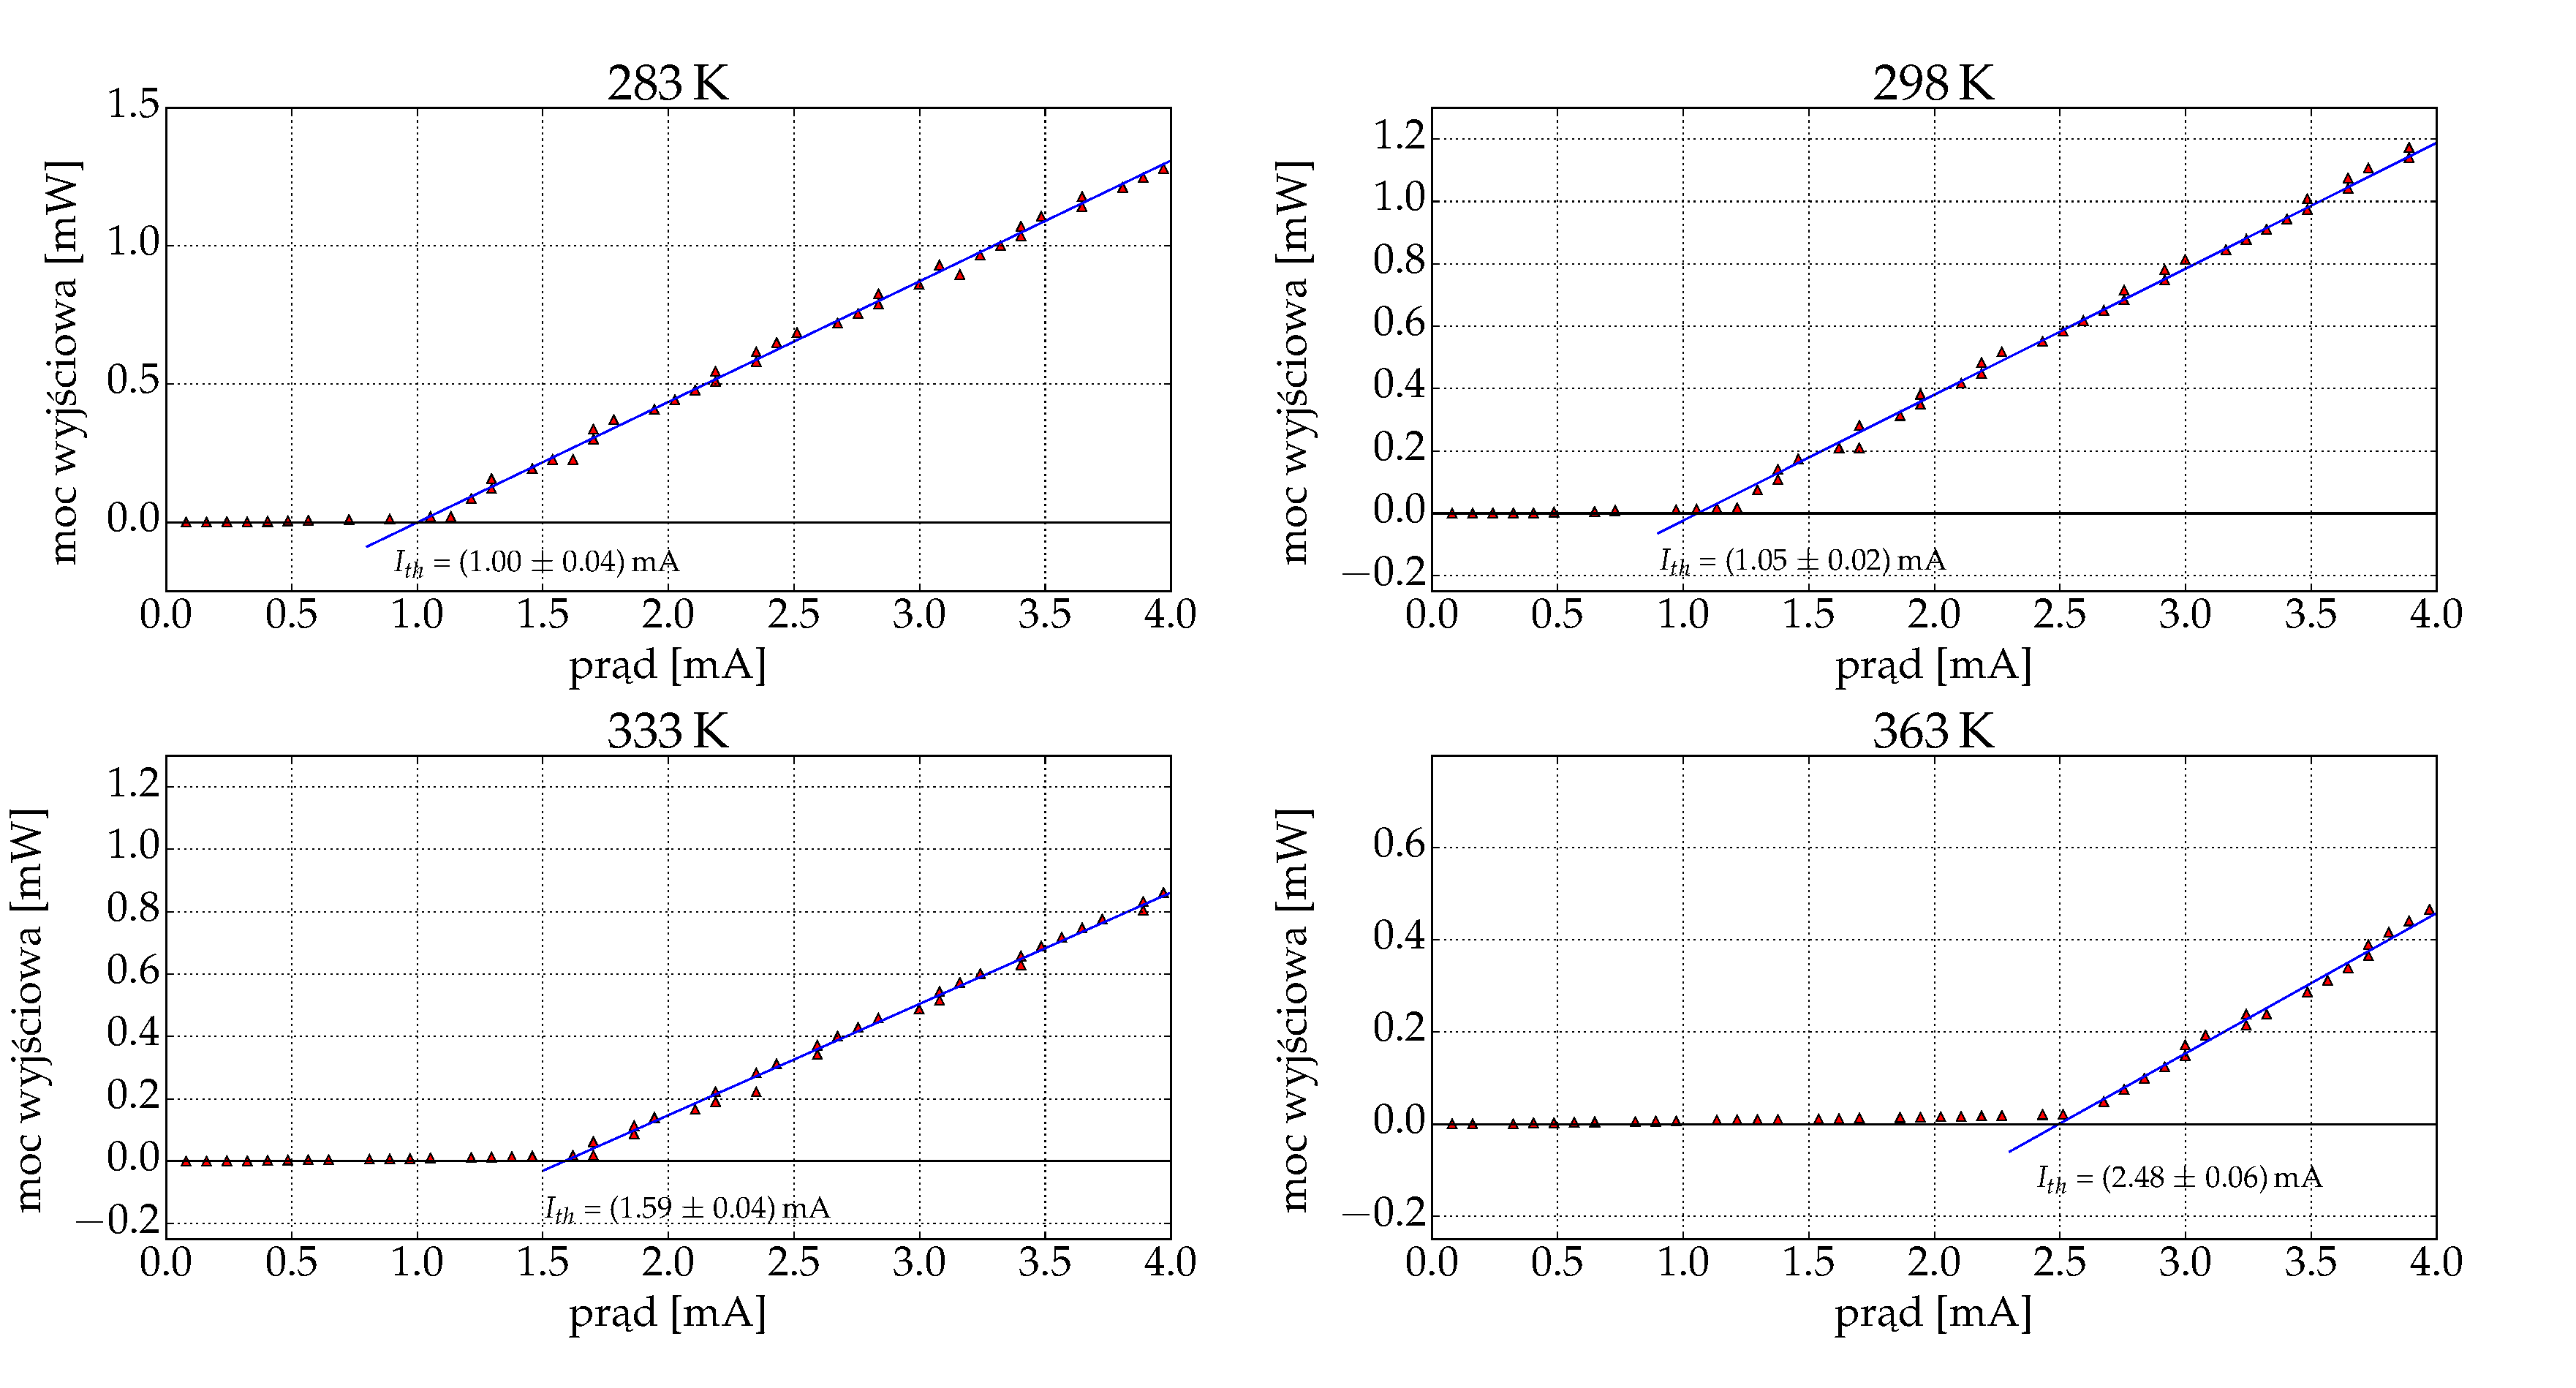
\includegraphics[scale=0.30]{plot980/plot_fit_i_th4.eps}
  \label{rys1}
  \caption{Wykres ilustrujący wyznaczanie prądu progow dla lasera VCSEL 980\,nm.}
\end{figure}
\begin{figure}
\center
  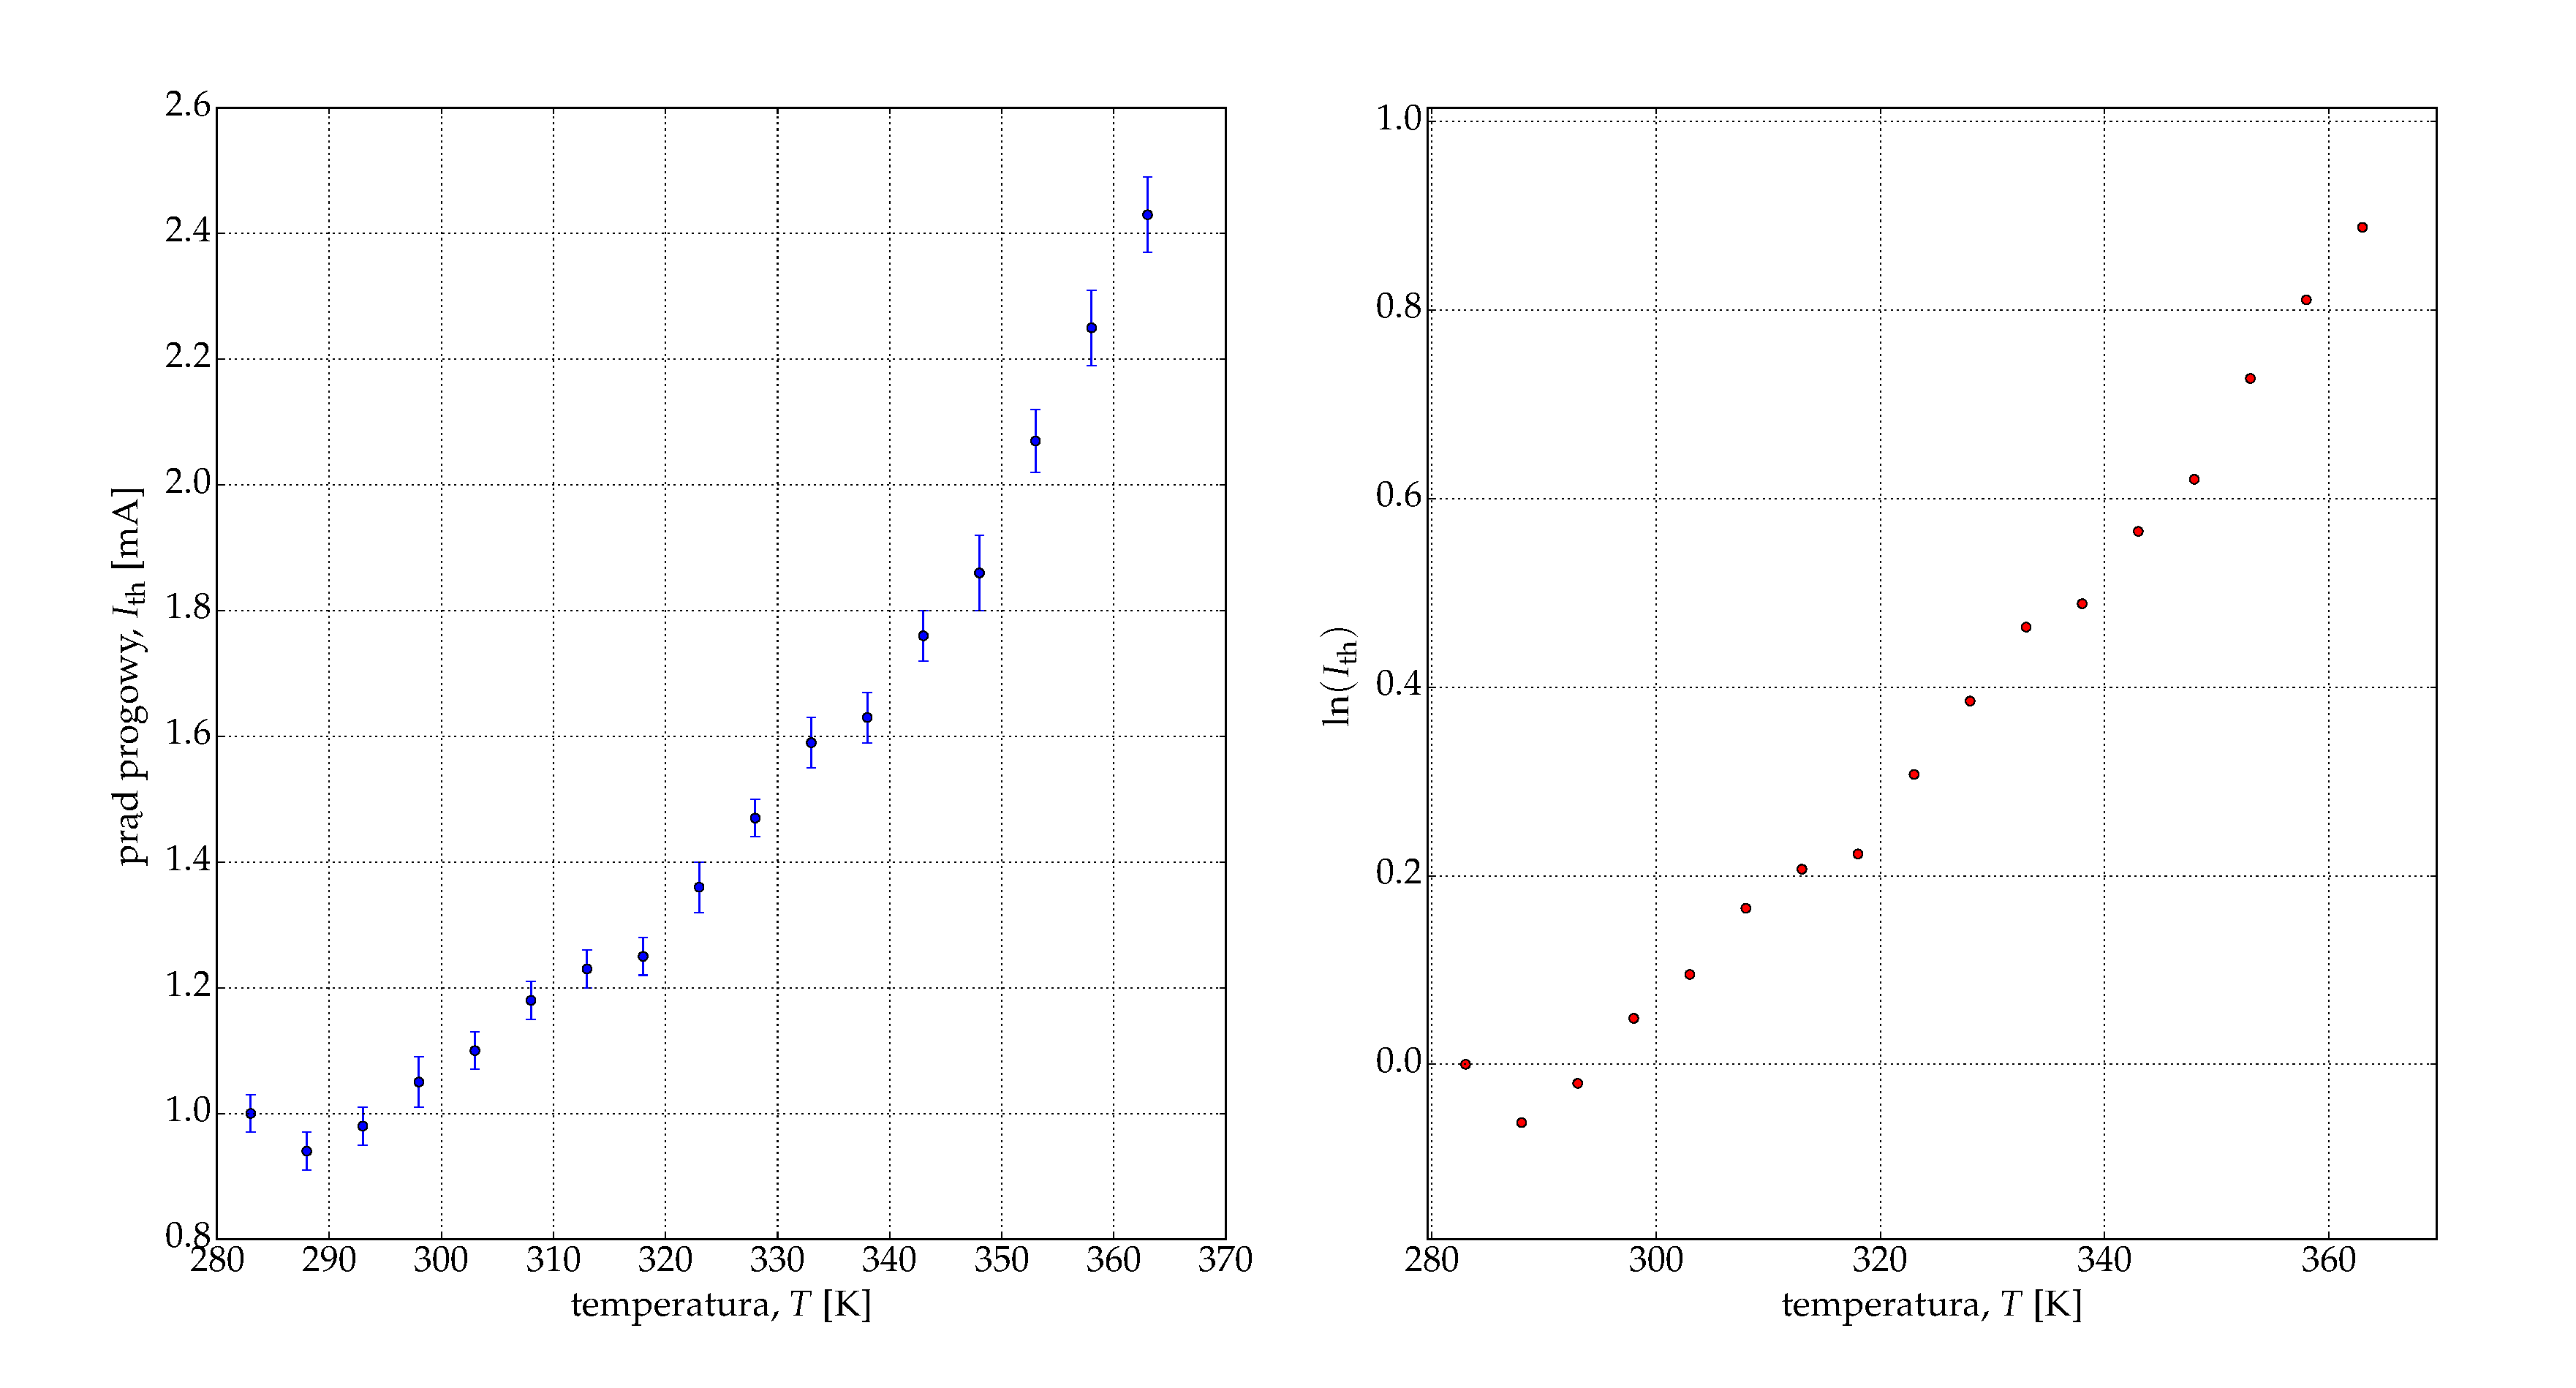
\includegraphics[scale=0.30]{plot980/plot_temp_i_th_log_lin.eps}
  \label{rys1}
  \caption{Wykres prądu progow od temperatury dla lasera VCSEL 980\,nm w skali liniowej oraz logarytmicznej.}
\end{figure}
\begin{figure}
\center
  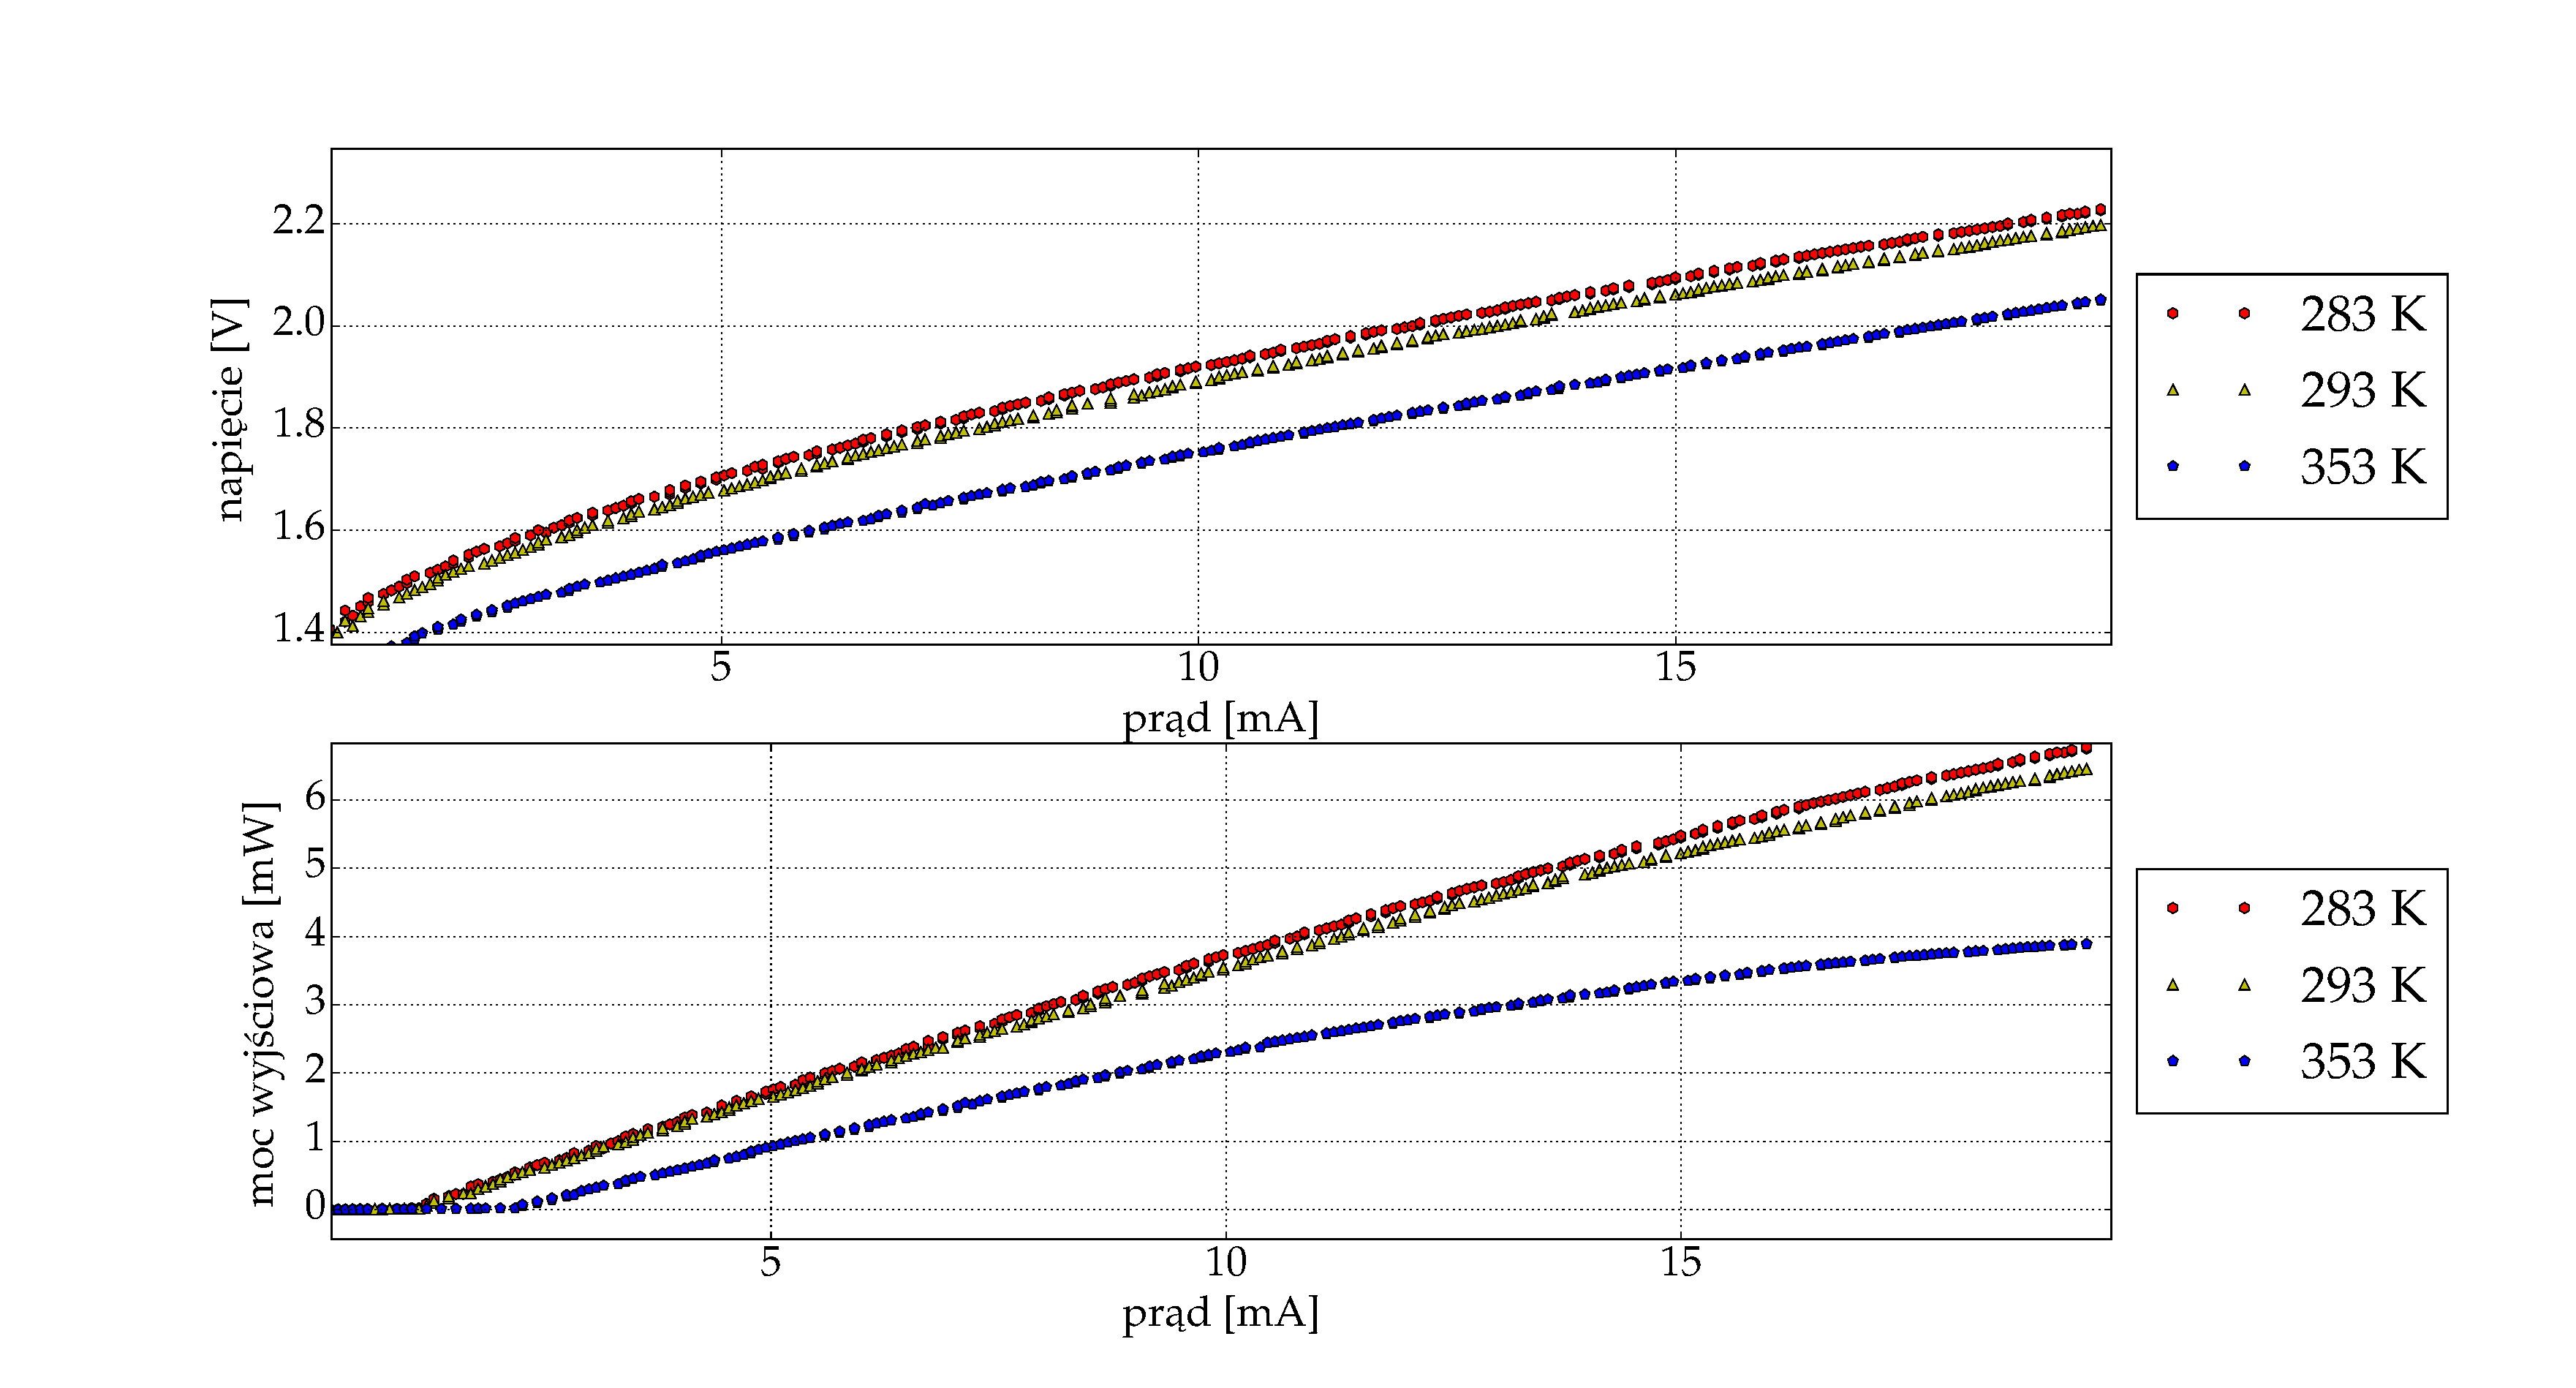
\includegraphics[scale=0.30]{plot980/plot_i_v_i_l.eps}
  \label{rys1}
  \caption{Wykres napięcia oraz mocy wyjściowej w fukcji prądu dla lasera VCSEL 980\,nm.}
\end{figure}
\begin{figure}
\center
  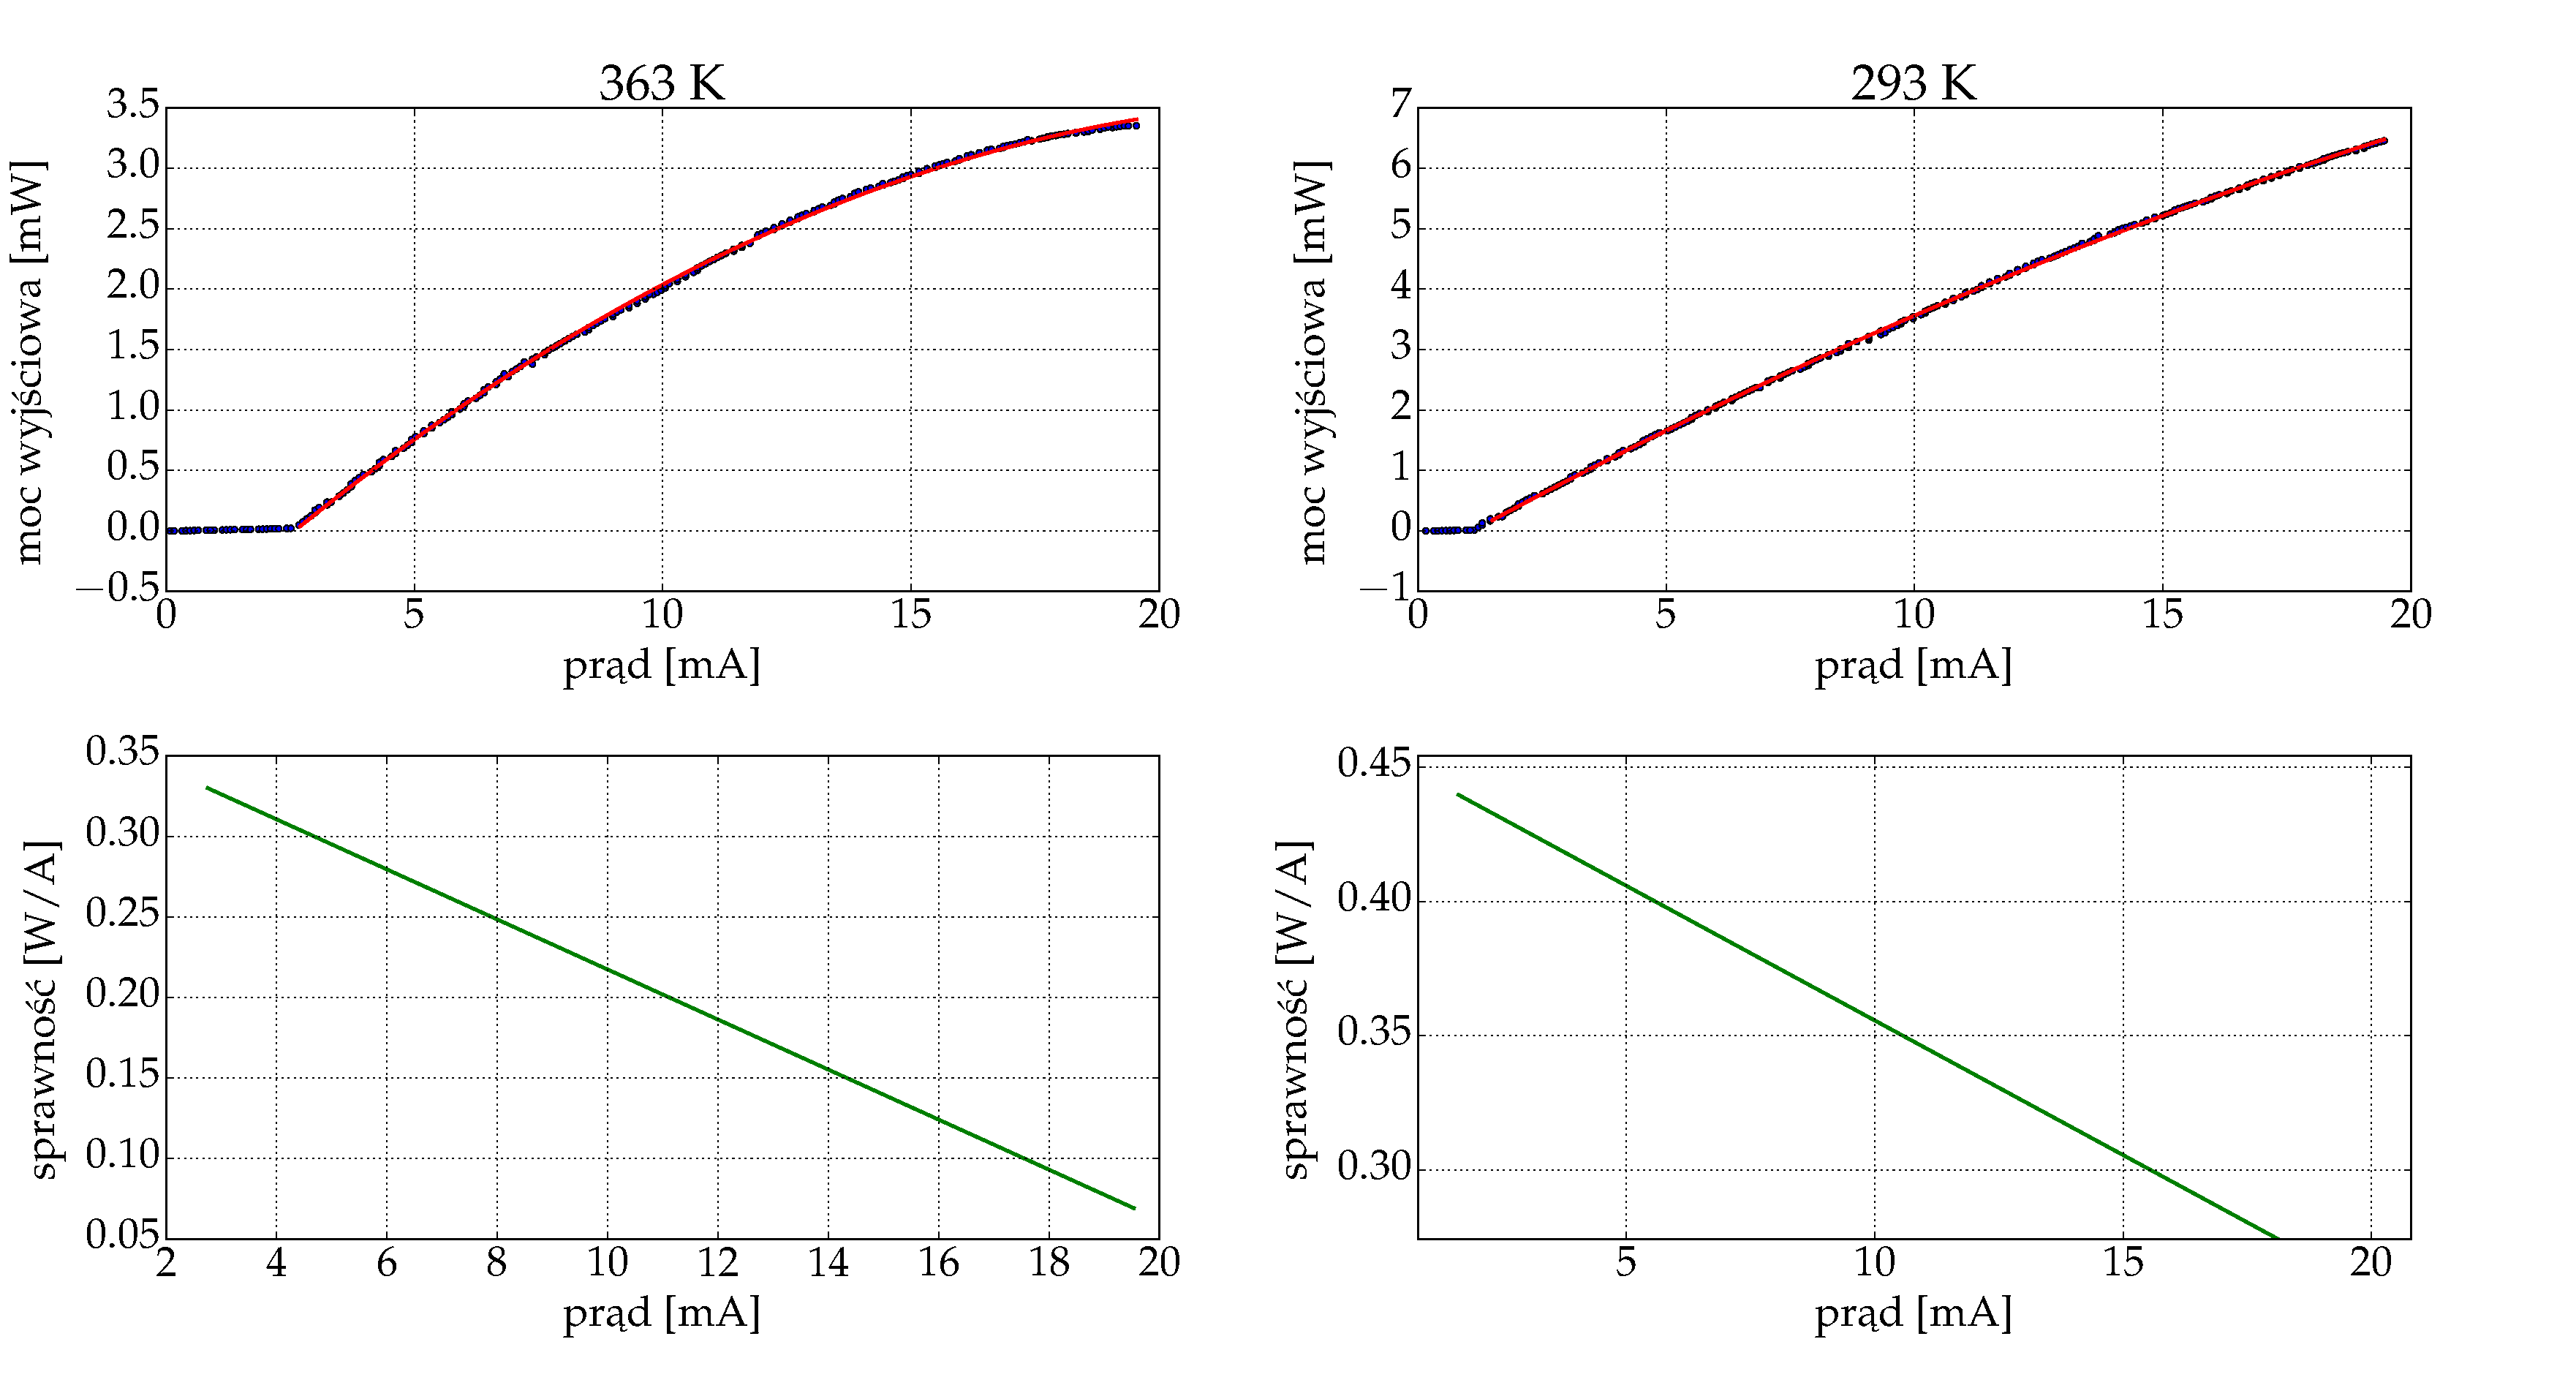
\includegraphics[scale=0.30]{plot980/plot_eff_via_current4.eps}
  \label{rys1}
  \caption{Wykres sprawności różnoczkowej dla lasera VCSEL 980\,nm w dwóch różnych temperaturach.}
\end{figure}
\begin{figure}
\center
  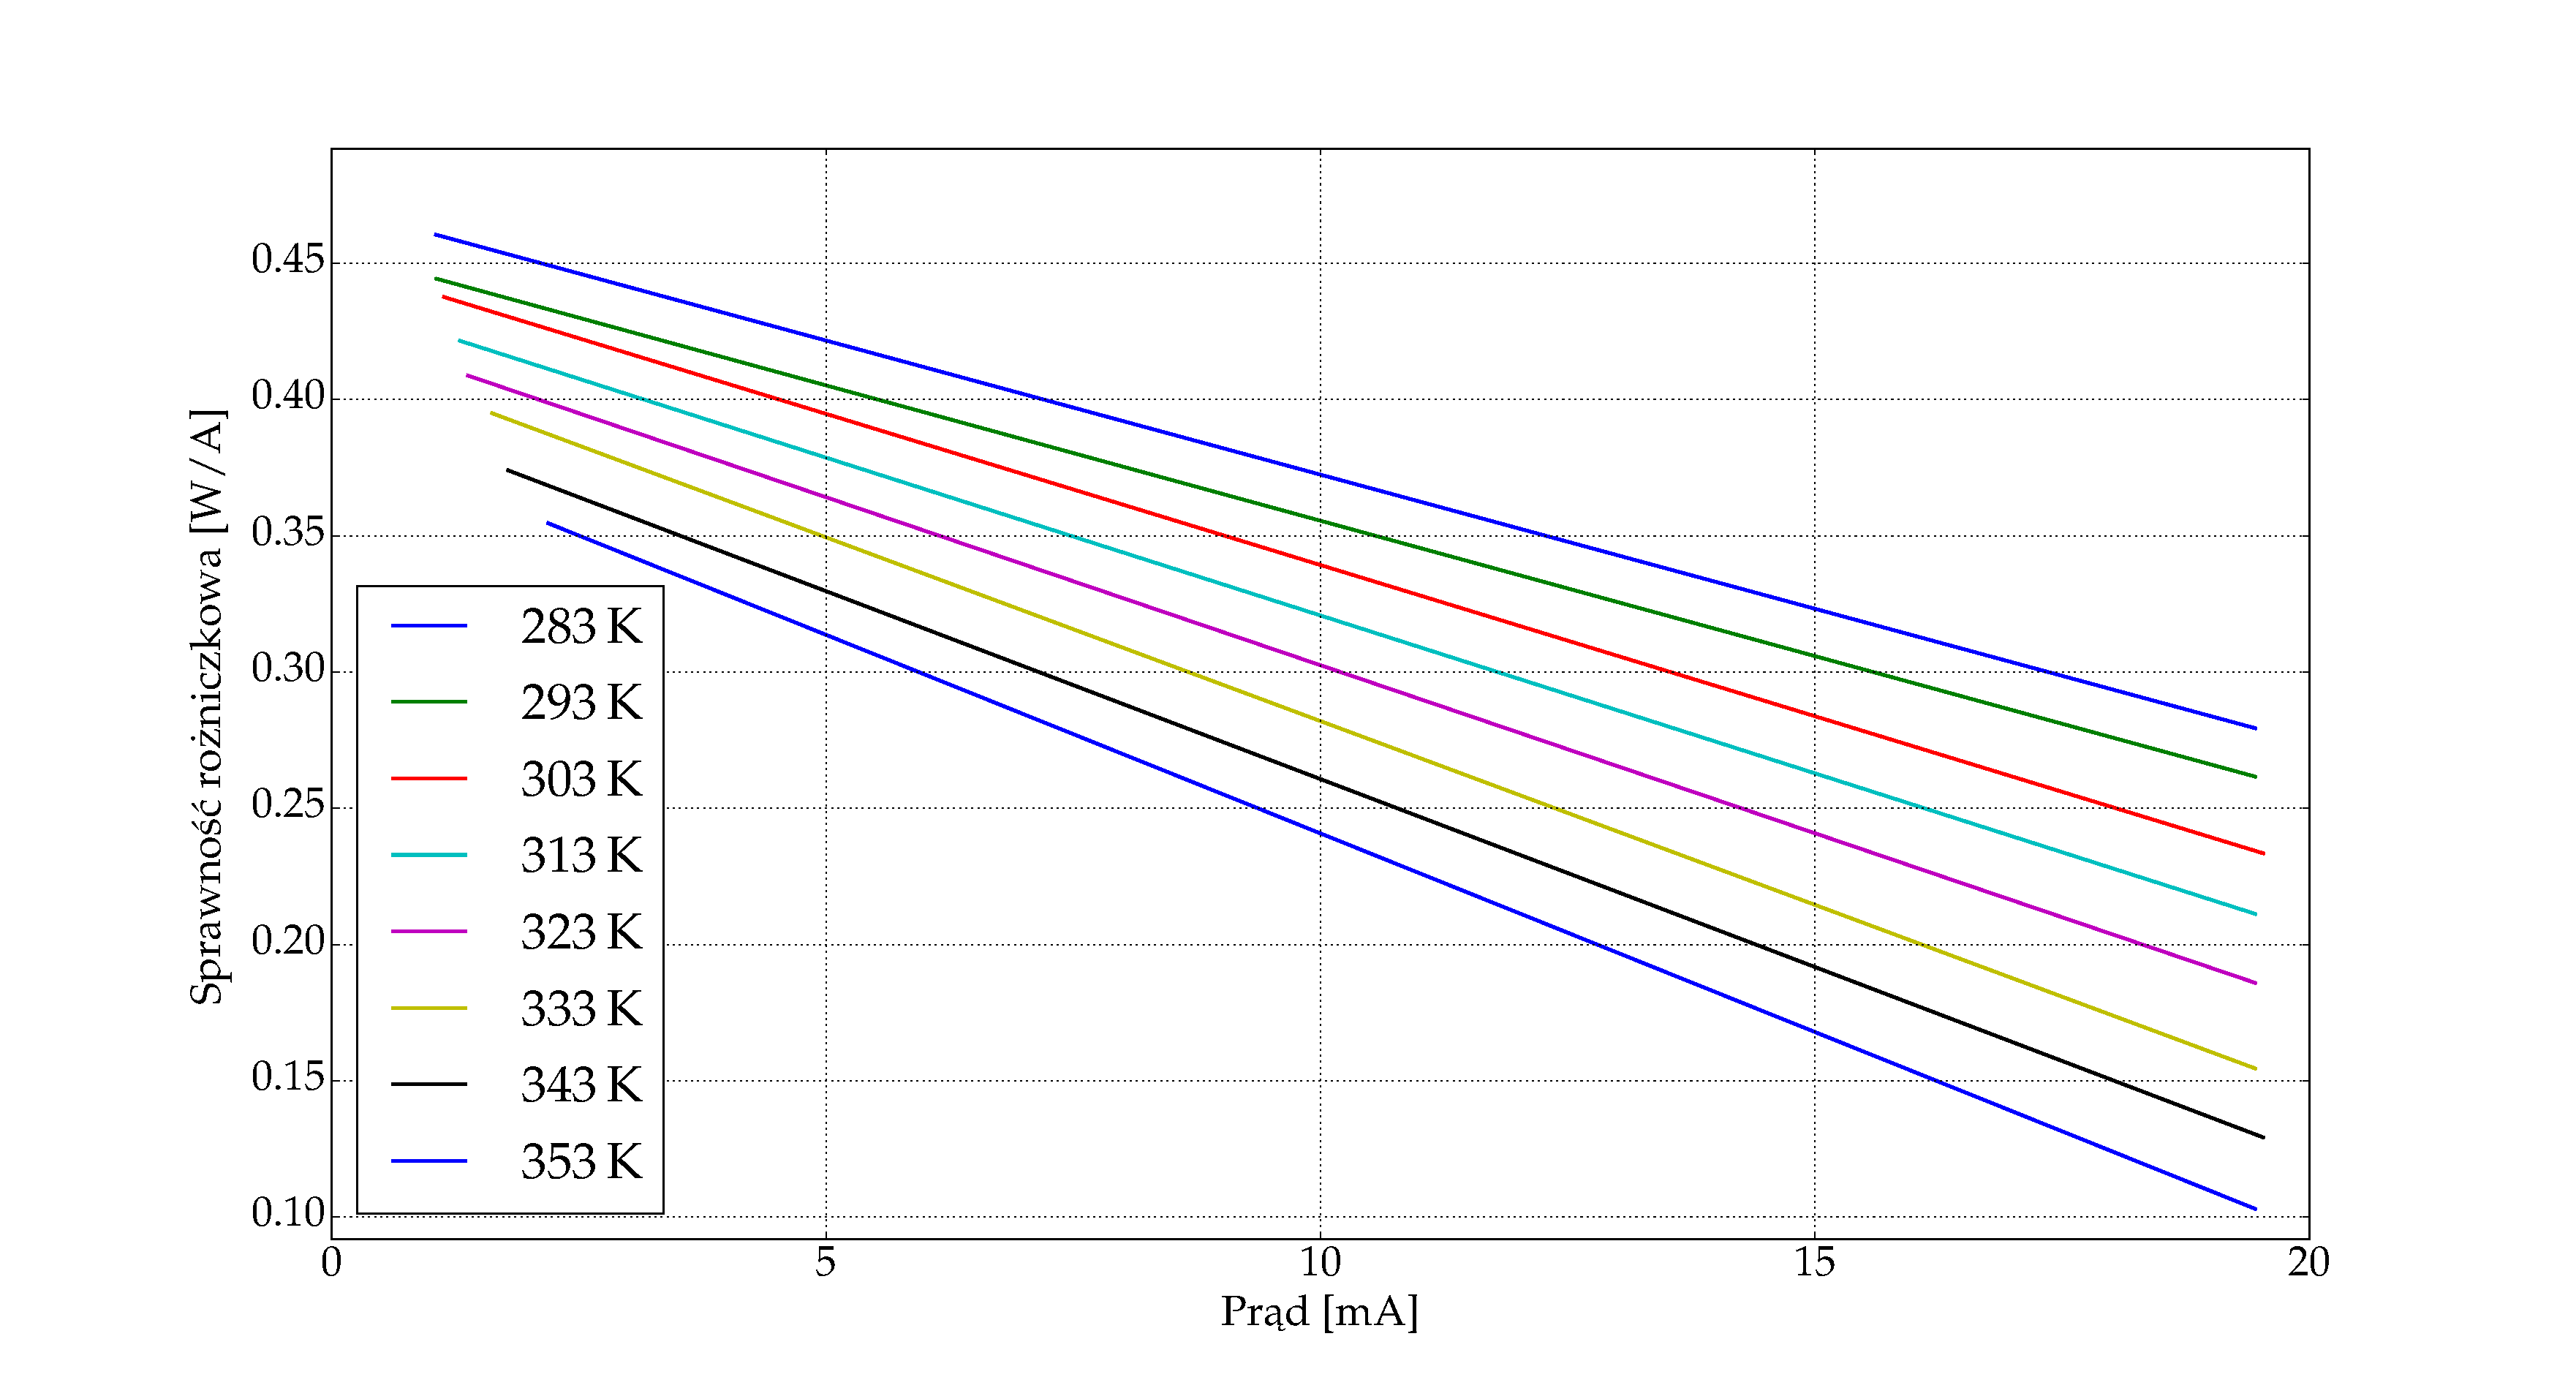
\includegraphics[scale=0.30]{plot980/plot_eff_via_current_all.eps}
  \label{rys1}
  \caption{Wykres sprawności różnoczkowej dla lasera VCSEL 980\,nm w różnych temperaturach.}
\end{figure}